\documentclass[border=3pt]{standalone}
% Preâmbulo compartilhado pelos diagramas TikZ da aula 4 de Navegação (Representação de Mapas)
\usepackage[T1]{fontenc}
\usepackage[utf8]{inputenc}
\usepackage{lmodern}
\usepackage{amsmath}
\usepackage{xcolor}
\usepackage{tikz}
\usetikzlibrary{arrows.meta,angles,quotes,decorations.pathmorphing,decorations.pathreplacing,calc,
                positioning,shapes.geometric,shapes.misc,backgrounds,fit,
                math}

% Paleta (mesma dos SVGs originais)
\definecolor{dblue}{HTML}{2A5B8C}
\definecolor{dorange}{HTML}{B3541E}
\definecolor{dgreen}{HTML}{4A7C59}
\definecolor{dred}{HTML}{9C4B4B}
\definecolor{dcream}{HTML}{F4F1EA}
\definecolor{dshade}{HTML}{DDD7C9}

% Função gaussiana (não normalizada por padrão de escala visual)
\pgfmathdeclarefunction{gauss}{3}{%
  \pgfmathparse{1/(#3*sqrt(2*pi))*exp(-((#1-#2)^2)/(2*#3^2))}%
}

% Estilos comuns (prefixo d... para não colidir com chaves internas do pgf)
\tikzset{
  >={Stealth[length=2mm]},
  dguide/.style={gray!55, dashed, line width=0.4pt},
  daxis/.style={gray!60, line width=0.7pt, ->},
  dbody/.style={fill=black!3, draw=black!80, line width=1pt},
  dacc/.style={draw=dblue, line width=1pt},
  dlbl/.style={black!55, font=\small},
  dsub/.style={black!45, font=\footnotesize},
  dstate/.style={circle, draw=black!80, fill=dcream, line width=1pt,
                 minimum size=17mm, font=\large, inner sep=1pt},
  dobs/.style={circle, draw=black!80, fill=dshade, line width=1pt,
               minimum size=14mm, font=\large, inner sep=1pt},
  dbox/.style={rounded corners=2pt, draw=black!80, fill=dcream, line width=1pt,
               align=center, inner sep=6pt},
  dop/.style={circle, draw=black!80, fill=white, line width=1pt,
              minimum size=6mm, inner sep=0pt, font=\small},
  dtrans/.style={->, dblue, line width=1pt},
  dmeas/.style={->, dorange, line width=1pt},
  dcurve/.style={line width=1pt, dblue},
  dcurveb/.style={line width=1.4pt, dorange},
}

\begin{document}
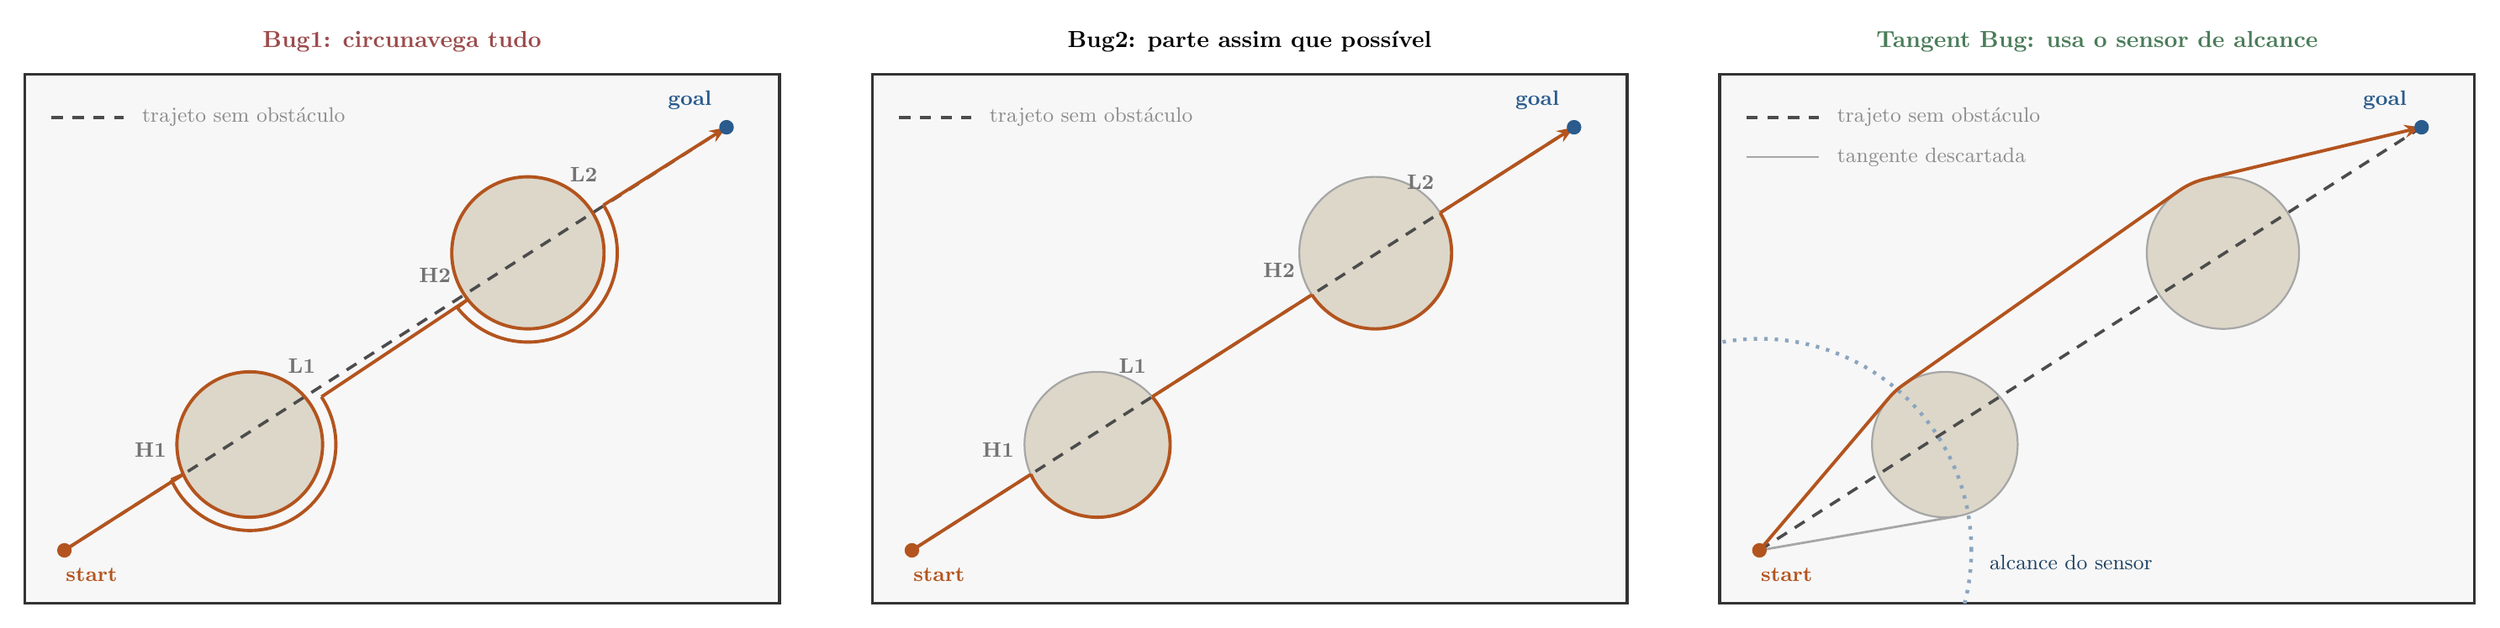
\begin{tikzpicture}[x=1cm,y=1cm]

  \begin{scope}[shift={(0,0)}]
    \draw[dbody, line width=1.2pt] (0,0) rectangle (11.4,8.0);
    \node[font=\bfseries\normalsize, dred] at (5.7,8.5) {Bug1: circunavega tudo};
    \fill[dshade, draw=black!35, line width=0.8pt] (3.40,2.40) circle (1.10);
    \fill[dshade, draw=black!35, line width=0.8pt] (7.60,5.30) circle (1.15);
    \draw[black!70, dash pattern=on 5pt off 4pt, line width=1.3pt] (0.600,0.800) -- (10.600,7.200);
    \draw[dcurveb] (0.600,0.800) -- (2.396,1.950);
    \draw[dcurveb] (2.396,1.950) arc (204.17:564.17:1.100);
    \draw[dcurveb] (2.396,1.950) -- (2.214,1.868);
    \draw[dcurveb] (2.214,1.868) arc (204.17:393.69:1.300);
    \draw[dcurveb] (4.482,3.121) -- (6.692,4.595);
    \draw[dcurveb] (6.692,4.595) arc (217.84:577.84:1.150);
    \draw[dcurveb] (6.692,4.595) -- (6.534,4.472);
    \draw[dcurveb] (6.534,4.472) arc (217.84:392.35:1.350);
    \draw[dcurveb, -{Stealth[length=2.6mm]}] (8.741,6.022) -- (10.600,7.200);
    \fill[dorange] (0.600,0.800) circle (0.11); \node[dorange,font=\small\bfseries,anchor=north west] at (0.500,0.650) {start};
    \fill[dblue] (10.600,7.200) circle (0.11); \node[dblue,font=\small\bfseries,anchor=south east] at (10.500,7.350) {goal};
    \node[dlbl,font=\small\bfseries] at (1.901,2.322) {H1};
    \node[dlbl,font=\small\bfseries] at (4.185,3.584) {L1};
    \node[dlbl,font=\small\bfseries] at (6.196,4.966) {H2};
    \node[dlbl,font=\small\bfseries] at (8.444,6.485) {L2};
    \draw[black!70, dash pattern=on 5pt off 4pt, line width=1.3pt] (0.4,7.35) -- (1.5,7.35);
    \node[dsub,font=\small,anchor=west] at (1.65,7.35) {trajeto sem obstáculo};
  \end{scope}

  \begin{scope}[shift={(12.8,0)}]
    \draw[dbody, line width=1.2pt] (0,0) rectangle (11.4,8.0);
    \node[font=\bfseries\normalsize] at (5.7,8.5) {Bug2: parte assim que possível};
    \fill[dshade, draw=black!35, line width=0.8pt] (3.40,2.40) circle (1.10);
    \fill[dshade, draw=black!35, line width=0.8pt] (7.60,5.30) circle (1.15);
    \draw[black!70, dash pattern=on 5pt off 4pt, line width=1.3pt] (0.600,0.800) -- (10.600,7.200);
    \draw[dcurveb] (0.600,0.800) -- (2.396,1.950);
    \draw[dcurveb] (2.396,1.950) arc (204.17:401.07:1.100);
    \draw[dcurveb] (4.229,3.123) -- (6.641,4.666);
    \draw[dcurveb] (6.641,4.666) arc (213.46:391.78:1.150);
    \draw[dcurveb, -{Stealth[length=2.6mm]}] (8.578,5.906) -- (10.600,7.200);
    \fill[dorange] (0.600,0.800) circle (0.11); \node[dorange,font=\small\bfseries,anchor=north west] at (0.500,0.650) {start};
    \fill[dblue] (10.600,7.200) circle (0.11); \node[dblue,font=\small\bfseries,anchor=south east] at (10.500,7.350) {goal};
    \node[dlbl,font=\small\bfseries] at (1.901,2.322) {H1};
    \node[dlbl,font=\small\bfseries] at (3.933,3.586) {L1};
    \node[dlbl,font=\small\bfseries] at (6.145,5.038) {H2};
    \node[dlbl,font=\small\bfseries] at (8.281,6.369) {L2};
    \draw[black!70, dash pattern=on 5pt off 4pt, line width=1.3pt] (0.4,7.35) -- (1.5,7.35);
    \node[dsub,font=\small,anchor=west] at (1.65,7.35) {trajeto sem obstáculo};
  \end{scope}


  % Painel C: Tangent Bug
  \begin{scope}[shift={(25.6,0)}]
    \draw[dbody, line width=1.2pt] (0,0) rectangle (11.4,8.0);
    \node[font=\bfseries\normalsize, dgreen] at (5.7,8.5) {Tangent Bug: usa o sensor de alcance};
    \fill[dshade, draw=black!35, line width=0.8pt] (3.40,2.40) circle (1.10);
    \fill[dshade, draw=black!35, line width=0.8pt] (7.60,5.30) circle (1.15);
    \draw[black!70, dash pattern=on 5pt off 4pt, line width=1.3pt] (0.600,0.800) -- (10.600,7.200);
    \begin{scope}
      \clip (0,0) rectangle (11.4,8.0);
      \draw[dblue!55!white, dash pattern=on 1.5pt off 3pt, line width=1.6pt] (0.600,0.800) circle (3.20);
    \end{scope}
    \draw[black!35, line width=1pt] (0.600,0.800) -- (3.587,1.316);
    \draw[dcurveb] (0.600,0.800) -- (2.561,3.112);
    \draw[dcurveb] (2.561,3.112) arc (139.69:125.19:1.100);
    \draw[dcurveb] (2.766,3.299) -- (6.937,6.240);
    \draw[dcurveb] (6.937,6.240) arc (125.19:103.45:1.150);
    \draw[dcurveb, -{Stealth[length=2.6mm]}] (7.332,6.418) -- (10.600,7.200);
    \fill[dorange] (0.600,0.800) circle (0.11); \node[dorange,font=\small\bfseries,anchor=north west] at (0.500,0.650) {start};
    \fill[dblue] (10.600,7.200) circle (0.11); \node[dblue,font=\small\bfseries,anchor=south east] at (10.500,7.350) {goal};
    \node[dblue!70!black,font=\small,anchor=west] at (3.95,0.62) {alcance do sensor};
    \draw[black!70, dash pattern=on 5pt off 4pt, line width=1.3pt] (0.4,7.35) -- (1.5,7.35);
    \node[dsub,font=\small,anchor=west] at (1.65,7.35) {trajeto sem obstáculo};
    \draw[black!35, line width=1pt] (0.4,6.75) -- (1.5,6.75);
    \node[dsub,font=\small,anchor=west] at (1.65,6.75) {tangente descartada};
  \end{scope}

\end{tikzpicture}
\end{document}
